\documentclass[12pt,a4paper]{article}

% Essential packages
\usepackage[utf8]{inputenc}
\usepackage[T1]{fontenc}
\usepackage{amsmath,amssymb,amsthm}
\usepackage{mathtools}
\usepackage{geometry}
\usepackage[colorlinks=true, linkcolor=leanblue, citecolor=leanblue, urlcolor=leanblue]{hyperref}
\usepackage{xcolor}
\usepackage{fancyhdr}
\usepackage{listings}
\usepackage{stmaryrd}
\usepackage{tikz}

\geometry{left=2.5cm, right=2.5cm, top=3cm, bottom=3cm}

% Colors
\definecolor{leanblue}{RGB}{0, 84, 166}
\definecolor{leangreen}{RGB}{0, 128, 0}

% Theorem environments
\theoremstyle{definition}
\newtheorem{definicao}{Definition}[section]
\newtheorem{exemplo}[definicao]{Example}
\theoremstyle{plain}
\newtheorem{teorema}[definicao]{Theorem}
\newtheorem{proposicao}[definicao]{Proposition}
\newtheorem{lema}[definicao]{Lemma}
\theoremstyle{remark}
\newtheorem{observacao}[definicao]{Remark}

% Commands
\newcommand{\sem}[1]{\llbracket #1 \rrbracket}
\newcommand{\defeq}{\coloneqq}

% Lean code environment
\lstdefinelanguage{Lean}{
  keywords={theorem, lemma, def, example, by, intro, exact, apply, rfl, simp, sorry, constructor, cases, induction, have, show, assume, fun, match, with, end, if, then, else, let, in, where, structure, class, instance, extends, namespace, variable, open, notation, inductive, deriving, calc, universe, Type, Prop},
  sensitive=true,
  comment=[l]{--},
  morecomment=[s]{/-}{-/},
  string=[b]",
}

\lstnewenvironment{leancode}{%
	\lstset{
		language=Lean,
		basicstyle=\ttfamily\small,
		keywordstyle=\color{leanblue}\bfseries,
		commentstyle=\color{leangreen}\itshape,
		breaklines=true,
		frame=single,
		xleftmargin=1em,
		xrightmargin=1em,
		literate=
		{α}{{$\alpha$}}1
		{β}{{$\beta$}}1
		{→}{{$\to$}}1
		{←}{{$\leftarrow$}}1
		{↔}{{$\leftrightarrow$}}1
		{≤}{{$\leq$}}1
		{≥}{{$\geq$}}1
		{≠}{{$\neq$}}1
		{∀}{{$\forall$}}1
		{∃}{{$\exists$}}1
		{¬}{{$\neg$}}1
		{∧}{{$\land$}}1
		{∨}{{$\lor$}}1
		{⦃}{{$\lbrace\mkern-4mu|$}}1
		{⦄}{{$|\mkern-4mu\rbrace$}}1
		{⊗}{{$\otimes$}}1
		{₁}{{$_1$}}1
		{₂}{{$_2$}}1
		{·}{{$\cdot$}}1,
	}%
}{}

% Header
\pagestyle{fancy}
\fancyhf{}
\lhead{Igor Strozzi}
\chead{Intuitionistic Type Theory and Lean}
\rhead{Supplementary}
\cfoot{\thepage}

\title{\textbf{Mereotopological Ontologies with Compositional Algebras}\\[0.5em]
\large A Formalization in Lean 4}
\author{Igor Strozzi\\
\small UFRJ --- Professor Francesco Noseda}
\date{2025-2}

\begin{document}
\maketitle

\begin{abstract}
We develop the mathematical foundations for formalizing mereotopological ontologies equipped with compositional algebras that function as deductive systems. The key insight is that Heyting algebras---the algebraic semantics for intuitionistic logic---provide the natural framework for such compositional structures. We present a complete, self-contained Lean 4 formalization.
\end{abstract}

\tableofcontents
\newpage

\section{Introduction}

Given a formal ontology $\mathcal{O}$ with mereotopological structure (part-whole relations and topological connection) and an algebra $\mathcal{A}$ acting on $\mathcal{O}$, we seek to formalize:
\begin{enumerate}
    \item The mereotopological structure of $\mathcal{O}$
    \item The algebraic structure of $\mathcal{A}$ as a Heyting algebra
    \item The action $\sem{\cdot} : \mathcal{O} \to A$ preserving relevant structure
    \item The deductive character emerging from the Heyting implication
\end{enumerate}

\section{Mereotopological Ontology}

\begin{definicao}[Mereotopological Ontology]
A \emph{mereotopological ontology} is a structure $\mathcal{O} = (O, \sqsubseteq, \mathsf{C})$ where:
\begin{itemize}
    \item $O$ is a non-empty set of \emph{concepts} or \emph{entities}
    \item $\sqsubseteq$ is a \emph{parthood} relation (partial order)
    \item $\mathsf{C}$ is a \emph{connection} relation (reflexive, symmetric)
\end{itemize}
satisfying the \emph{mereotopological coherence axiom}:
$$
x \sqsubseteq y \implies \mathsf{C}(x, y)
$$
\end{definicao}

The parthood relation $\sqsubseteq$ satisfies:
\begin{itemize}
    \item \textbf{Reflexivity:} $\forall x.\, x \sqsubseteq x$
    \item \textbf{Transitivity:} $x \sqsubseteq y \land y \sqsubseteq z \implies x \sqsubseteq z$
    \item \textbf{Antisymmetry:} $x \sqsubseteq y \land y \sqsubseteq x \implies x = y$
\end{itemize}

\begin{definicao}[Derived Mereotopological Relations]
From the primitive relations, we define:
\begin{align*}
    \mathsf{PP}(x, y) &\defeq x \sqsubseteq y \land x \neq y && \text{(proper parthood)} \\
    \mathsf{O}(x, y) &\defeq \exists z.\, z \sqsubseteq x \land z \sqsubseteq y && \text{(overlap)} \\
    \mathsf{D}(x, y) &\defeq \neg \mathsf{O}(x, y) && \text{(disjointness)} \\
    \mathsf{EC}(x, y) &\defeq \mathsf{C}(x, y) \land \mathsf{D}(x, y) && \text{(external connection)}
\end{align*}
\end{definicao}

\begin{observacao}
The connection relation $\mathsf{C}$ captures topological adjacency without requiring shared parts. Two concepts can be externally connected (touching) without overlapping---a crucial distinction for spatial and conceptual reasoning.
\end{observacao}

\section{Heyting Algebras as Compositional Algebras}

Recall that a Heyting algebra provides algebraic semantics for intuitionistic logic.

\begin{definicao}[Heyting Algebra]
A \emph{Heyting algebra} is a bounded distributive lattice $\mathcal{H} = (H, \sqcup, \sqcap, \Rightarrow, 0, 1)$ such that for all $a, b \in H$, the \emph{relative pseudo-complement} $a \Rightarrow b$ exists, characterized by the \textbf{adjunction property}:
$$
c \sqcap a \leq b \iff c \leq a \Rightarrow b
$$
\end{definicao}

\begin{teorema}[Completeness]
For intuitionistic propositional logic:
$$
\Gamma \vdash \varphi \iff \Gamma \models \varphi
$$
where $\Gamma \models \varphi$ means: for every Heyting algebra $\mathcal{H}$ and valuation $v$, if $\mathcal{H}, v \models \Gamma$ then $\mathcal{H}, v \models \varphi$.
\end{teorema}

\subsection{Compositional Algebra Structure}

We interpret the Heyting algebra operations as conceptual composition operators:

\begin{center}
\begin{tabular}{cll}
    \textbf{Operation} & \textbf{Notation} & \textbf{Interpretation} \\
    \hline
    Meet & $a \sqcap b$ & Conceptual conjunction/composition \\
    Join & $a \sqcup b$ & Conceptual disjunction/choice \\
    Implication & $a \Rightarrow b$ & Conceptual entailment \\
    Negation & $\sim a = a \Rightarrow 0$ & Conceptual complement \\
    Top & $1$ & Universal concept \\
    Bottom & $0$ & Empty/impossible concept \\
\end{tabular}
\end{center}

\begin{definicao}[Derivability]
In a compositional algebra $\mathcal{A}$, we define the \emph{derivability relation}:
$$
a \vdash_{\mathcal{A}} b \defeq a \sqcap b = a
$$
This is equivalent to $a \leq b$ in the underlying order.
\end{definicao}

\begin{proposicao}
Derivability forms a preorder:
\begin{enumerate}
    \item \textbf{Reflexivity:} $a \vdash_{\mathcal{A}} a$ (since $a \sqcap a = a$)
    \item \textbf{Transitivity:} $a \vdash_{\mathcal{A}} b$ and $b \vdash_{\mathcal{A}} c$ implies $a \vdash_{\mathcal{A}} c$
\end{enumerate}
\end{proposicao}

\section{The Ontological Algebra}

\begin{definicao}[Ontological Algebra]
An \emph{ontological algebra} is a triple $(\mathcal{O}, \mathcal{A}, \sem{\cdot})$ where:
\begin{itemize}
    \item $\mathcal{O} = (O, \sqsubseteq, \mathsf{C})$ is a mereotopological ontology
    \item $\mathcal{A}$ is a Heyting algebra (compositional algebra)
    \item $\sem{\cdot} : O \to A$ is an \emph{interpretation function}
\end{itemize}
satisfying:
\begin{enumerate}
    \item \textbf{Monotonicity:} $c_1 \sqsubseteq c_2 \implies \sem{c_1} \leq \sem{c_2}$
    \item \textbf{Connection non-triviality:} $\mathsf{C}(c_1, c_2) \implies \sem{c_1} \sqcap \sem{c_2} \neq 0$
\end{enumerate}
\end{definicao}

\begin{definicao}[Fundamental Operations]
Given concepts $C_1, C_2 \in O$, we define:
\begin{align*}
    C_1 \triangleright C_2 &\defeq \sem{C_1} \sqcap \sem{C_2} && \text{(combination)} \\
    C_1 \multimap C_2 &\defeq \sem{C_1} \Rightarrow \sem{C_2} && \text{(conceptual implication)}
\end{align*}
\end{definicao}

\subsection{Key Theorems}

\begin{teorema}[Parthood Implies Derivability]
If $c_1 \sqsubseteq c_2$ in $\mathcal{O}$, then:
$$
\sem{c_1} \sqcap \sem{c_2} = \sem{c_1}
$$
That is, $\sem{c_1} \vdash_{\mathcal{A}} \sem{c_2}$.
\end{teorema}

\begin{proof}
By monotonicity, $\sem{c_1} \leq \sem{c_2}$. Then:
$$
\sem{c_1} \sqcap \sem{c_2} \leq \sem{c_1} \leq \sem{c_2}
$$
so $\sem{c_1} \sqcap \sem{c_2} \leq \sem{c_1}$. Conversely, $\sem{c_1} \leq \sem{c_1} \sqcap \sem{c_2}$ since $\sem{c_1} \leq \sem{c_1}$ and $\sem{c_1} \leq \sem{c_2}$.
\end{proof}

\begin{teorema}[Overlap Non-Triviality]
If $\mathsf{O}(c_1, c_2)$ in $\mathcal{O}$, then $c_1 \triangleright c_2 \neq 0$.
\end{teorema}

\begin{proof}
From $\mathsf{O}(c_1, c_2)$, there exists $z$ with $z \sqsubseteq c_1$ and $z \sqsubseteq c_2$. By monotonicity, $\sem{z} \leq \sem{c_1}$ and $\sem{z} \leq \sem{c_2}$, so $\sem{z} \leq \sem{c_1} \sqcap \sem{c_2}$. By $\mathsf{C}$-reflexivity, $\mathsf{C}(z, z)$ holds, so by connection non-triviality, $\sem{z} \sqcap \sem{z} = \sem{z} \neq 0$. Thus $c_1 \triangleright c_2 \geq \sem{z} \neq 0$.
\end{proof}

\begin{teorema}[Modus Ponens for Concepts]
For any $c_1, c_2 \in O$:
$$
\sem{c_1} \sqcap (c_1 \multimap c_2) \leq \sem{c_2}
$$
\end{teorema}

\begin{proof}
This is the Heyting algebra property: $a \sqcap (a \Rightarrow b) \leq b$.
\end{proof}

\section{Connection to Topological Semantics}

Open sets of a topological space form a Heyting algebra, providing a canonical model.

\begin{proposicao}[Topological Heyting Algebra]
Let $\mathcal{T}$ be a topological space. Then $\mathcal{H} = (\mathcal{O}(\mathcal{T}), \cup, \cap, \Rightarrow, \emptyset, \mathcal{T})$ is a Heyting algebra where:
\begin{align*}
    A \Rightarrow B &= \mathrm{Int}(-A \cup B) \\
    \sim A &= \mathrm{Int}(-A)
\end{align*}
\end{proposicao}

\begin{exemplo}[Peirce's Law Failure]
Consider $\mathcal{H} = \mathcal{O}(\mathbb{R})$ with $v(p) = \mathbb{R} \setminus \{0\}$ and $v(q) = \emptyset$. Then:
$$
\sem{(p \to q) \to p}_v = \mathrm{Int}(\emptyset \cup (\mathbb{R} \setminus \{0\})) = \mathbb{R} \setminus \{0\}
$$
So $\sem{((p \to q) \to p) \to p}_v = \mathbb{R} \setminus \{0\} \neq \mathbb{R}$.

\textbf{Ontologically:} Peirce's law fails because we cannot constructively obtain $p$ merely from knowing that ``if $p$ implied $q$, then $p$ would hold.''
\end{exemplo}

\section{The Three-Element Example}

Consider the three-element chain $\mathbf{3} = \{0 < a < 1\}$:

\begin{center}
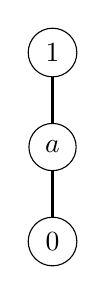
\begin{tikzpicture}[scale=0.8]
    \node[circle, draw, minimum size=6mm] (0) at (0,0) {$0$};
    \node[circle, draw, minimum size=6mm] (a) at (0,1.5) {$a$};
    \node[circle, draw, minimum size=6mm] (1) at (0,3) {$1$};
    \draw[thick] (0) -- (a) -- (1);
\end{tikzpicture}
\end{center}

The operations are:
\begin{center}
\begin{tabular}{c|ccc}
    $\sqcap$ & 0 & $a$ & 1 \\
    \hline
    0 & 0 & 0 & 0 \\
    $a$ & 0 & $a$ & $a$ \\
    1 & 0 & $a$ & 1
\end{tabular}
\qquad
\begin{tabular}{c|ccc}
    $\Rightarrow$ & 0 & $a$ & 1 \\
    \hline
    0 & 1 & 1 & 1 \\
    $a$ & 0 & 1 & 1 \\
    1 & 0 & $a$ & 1
\end{tabular}
\end{center}

\begin{observacao}
Note that $\sim a = a \Rightarrow 0 = 0$, but $\sim\sim a = 0 \Rightarrow 0 = 1 \neq a$. This demonstrates the failure of double negation elimination in intuitionistic logic.
\end{observacao}

\section{Lean 4 Formalization}

The complete formalization is self-contained, building all structures from first principles.

\subsection{Algebraic Foundations}

\begin{leancode}
class PartialOrder' (α : Type u) where
  le : α → α → Prop
  le_refl : ∀ a, le a a
  le_trans : ∀ {a b c}, le a b → le b c → le a c
  le_antisymm : ∀ {a b}, le a b → le b a → a = b

class HeytingAlgebra (α : Type u) extends BoundedLattice α where
  himp : α → α → α
  le_himp_iff : ∀ {a b c}, le (inf a b) c ↔ le a (himp b c)
\end{leancode}

\subsection{Mereotopological Ontology}

\begin{leancode}
class MereotopologicalOntology (O : Type u) where
  partOf : O → O → Prop
  C : O → O → Prop
  partOf_refl : ∀ x, partOf x x
  partOf_trans : ∀ {x y z}, partOf x y → partOf y z → partOf x z
  partOf_antisymm : ∀ {x y}, partOf x y → partOf y x → x = y
  C_refl : ∀ x, C x x
  C_symm : ∀ {x y}, C x y → C y x
  part_connected : ∀ {x y}, partOf x y → C x y
\end{leancode}

\subsection{The Ontological Algebra}

\begin{leancode}
class OntologicalAlgebra (O : Type u) (A : Type v)
    [MereotopologicalOntology O] [CompositionalAlgebra A] where
  interp : O → A
  interp_mono : ∀ {c₁ c₂}, partOf c₁ c₂ → interp c₁ ≤ interp c₂
  connected_nontrivial : ∀ {c₁ c₂}, C c₁ c₂ → 
    inf (interp c₁) (interp c₂) ≠ bot
\end{leancode}

\subsection{Key Theorem in Lean}

\begin{leancode}
theorem partOf_derives {c₁ c₂ : O}
    (h : MereotopologicalOntology.partOf c₁ c₂) :
    ⦃c₁⦄ ⊗ ⦃c₂⦄ = ⦃c₁⦄ := by
  apply le_antisymm
  · exact inf_le_left ⦃c₁⦄ ⦃c₂⦄
  · exact le_inf (le_refl ⦃c₁⦄) (interp_mono h)
\end{leancode}

\section{Philosophical Remarks}

The connection between mereotopological ontology and Heyting algebras illuminates deep correspondences:

\begin{enumerate}
    \item \textbf{Constructive Ontology:} Just as intuitionistic logic requires constructive evidence for assertions, ontological composition requires explicit witnesses (the overlap relation requires a common part).
    
    \item \textbf{Failure of Classical Duality:} The asymmetry between $\varphi \to \neg\neg\varphi$ (valid) and $\neg\neg\varphi \to \varphi$ (not valid) mirrors the asymmetry in mereotopology: parthood implies connection, but connection does not imply overlap.
    
    \item \textbf{Topological Intuition:} Interpreting concepts as open sets provides geometric intuition. A concept ``close to being true'' (like $\mathbb{R} \setminus \{0\}$) is not the same as being true ($\mathbb{R}$)---the boundary matters.
    
    \item \textbf{Compositional Semantics:} The adjunction $a \sqcap b \leq c \Leftrightarrow a \leq b \Rightarrow c$ captures the essence of compositional reasoning.
\end{enumerate}

\begin{observacao}[BHK Interpretation]
Under the BHK interpretation, a construction of $\varphi_1 \to \varphi_2$ is a method transforming constructions of $\varphi_1$ into constructions of $\varphi_2$. In our ontological setting:
$$
c_1 \multimap c_2 = \sem{c_1} \Rightarrow \sem{c_2}
$$
represents the ``conceptual method'' for deriving $c_2$ from $c_1$.
\end{observacao}

\section{Conclusion}

We have established a rigorous framework connecting:
\begin{itemize}
    \item \textbf{Mereotopology:} Part-whole and connection relations on concepts
    \item \textbf{Heyting Algebras:} The algebraic semantics of intuitionistic logic
    \item \textbf{Compositional Reasoning:} Deductive structure via the implication operation
    \item \textbf{Lean 4 Formalization:} Machine-checked proofs of the core theorems
\end{itemize}

The Heyting algebra structure naturally captures the intuitionistic character of ontological reasoning: we cannot assert properties of concepts without constructive justification, and the composition of concepts must respect the underlying mereotopological structure.

\section*{References}

\begin{enumerate}
    \item Sørensen, M.H. \& Urzyczyn, P. \textit{Lectures on the Curry-Howard Isomorphism}. Chapter 2: Intuitionistic Logic.
    \item Casati, R. \& Varzi, A.C. \textit{Parts and Places: The Structures of Spatial Representation}. MIT Press, 1999.
    \item Heyting, A. \textit{Intuitionism: An Introduction}. North-Holland, 1956.
\end{enumerate}

\end{document}
